\section{Deconvolution}
Our methods developped for the train won't work properly
without modification since they will try to deblur the background
which is not blurred.

The first thing we can do to adapt them is to just use them
on the subimage talked about in the section~\ref{sec:fg}.
This is the subimage around the shape we want to deblur
like the \figref{car-connected},
\figref{car-focusdiff} and \figref{car-focusdiffconnected}.

We could also only change pixels that are part of the solid
shape filled by the flood-fill.
This is the shaped represented by the
\figref{car-connected}.
That is how we have modified Wiener.

We could also do deeper adaptations of our methods.
That is what we have tried to do with Lucy-Richardson.
That is an advantage of this algorithm that we have already
talked about.
In addition to being the MLE of a poisson model,
it can also be viewed more intuitively.
By the way,
\cite{richardson1972bayesian} and \cite{lucy1974iterative}
are more based on the intuitive understanding and that is
only after, as we have seen that the link between poisson
was made.

The section~\ref{sec:lucy-intuitive} shows how to understand
it intuitively.

\subsection{Lucy-Richardson}
\subsubsection{select-lucy}
The first adaptation is a variant of what we have done
with Wiener that exploits the iterative approach of Lucy-Richardson.
Instead of doing the whole Lucy-Richardson process and then
only updating the foreground shape of the figure~\figref{car-connected}.
We can do it at each iteration.
That looks like the ``crop-lucy'' methods since when we do
$h * f_k$ in the iteration, we use a fixed value beyond the borders
which is the value of the image out of the foreground shape.
If the foreground estimate has all the foreground,
that should be unblurred background so we do not need approximation
this time.
However, in the $h * f_k$, a pixel on the border will be influenced
by the pixels of the background besides it and not only below it.
If $L$ is large and the background changes a lot, that can
creates a lot of problems on the borders.

We can see the effect of ``select-lucy'' on a rectangle blurred
on a background with the \figref{dontpanic_40-0_2_1-100_zoom}.
We can see that the background shape found is a bit bigger than the
real shape.
Since we want to be sure to have at least the foreground for
the flood-fill to work, it is an expected behavior of our algorithm
to have more than the background.
We can see the expected little problems at the borders that we
have just talked about.

\begin{myfig}{lucy-zooms}{Zooms}
  \begin{myfigsub}{dontpanic_40-0_2_1-100_zoom}
    {Zoom}{0.48}
    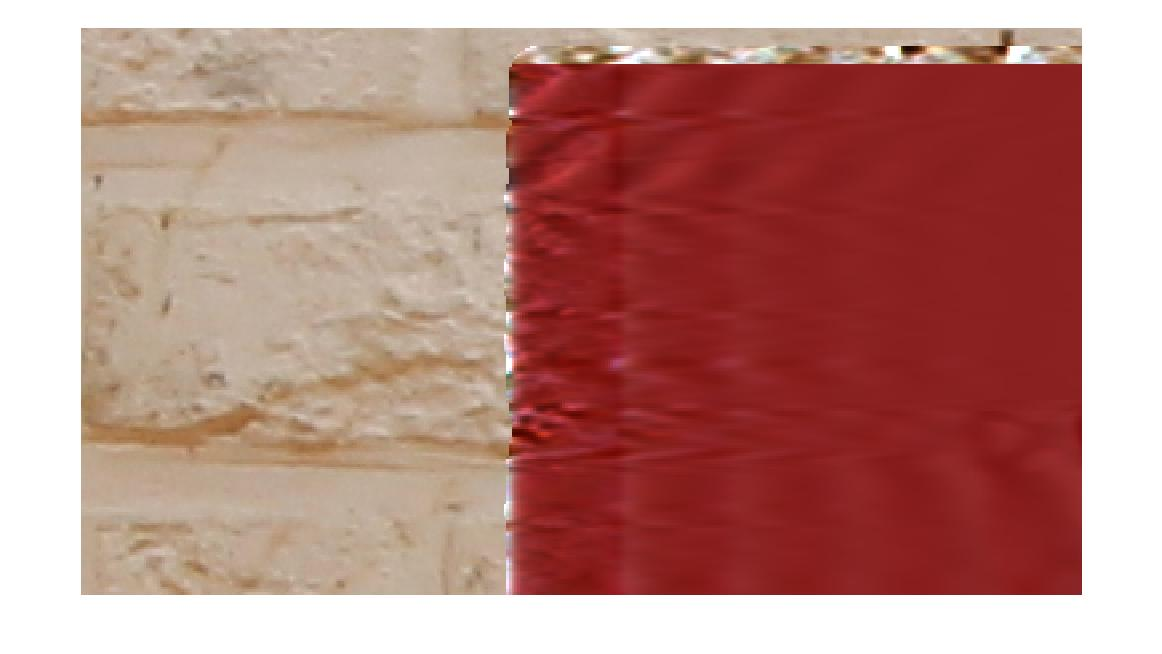
\includegraphics[width=\textwidth]{dontpanic-40-0_2_1-100_zoom.jpg}
  \end{myfigsub}
  \begin{myfigsub}{dontpanic_40-0_2_1-100_zoom}
    {Zoom}{0.48}
    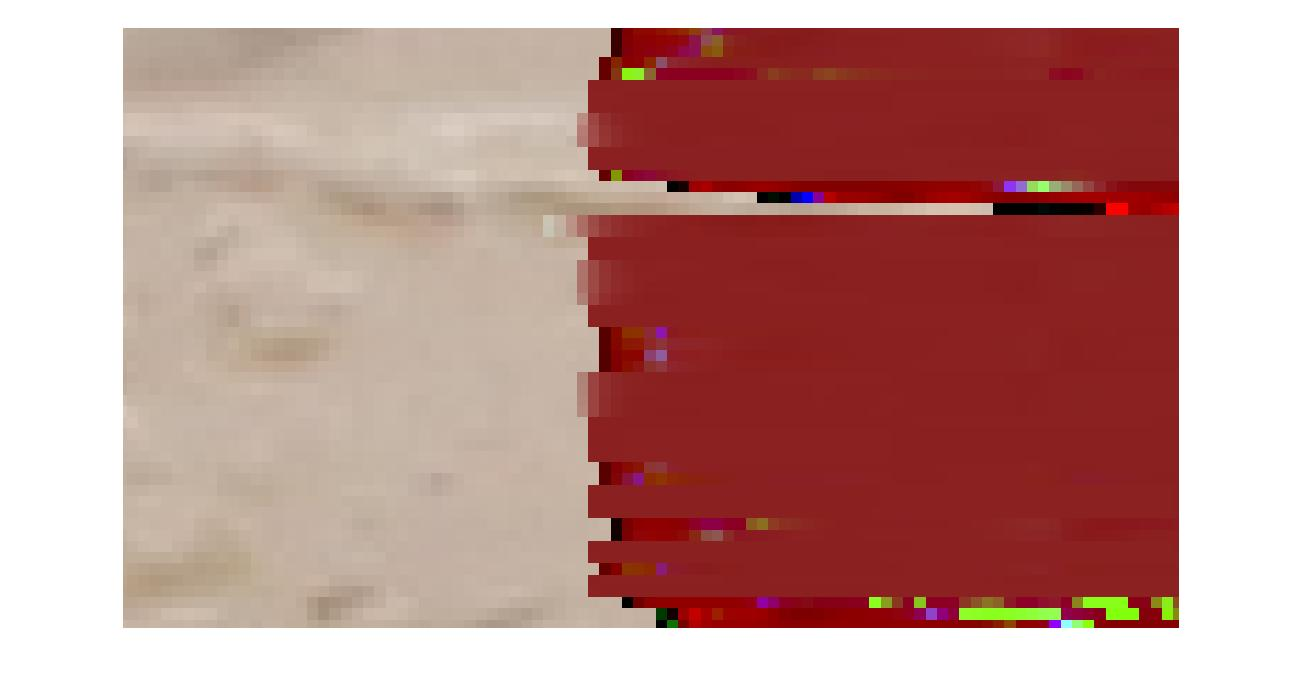
\includegraphics[width=\textwidth]{dontpanic-40_0-2_2-100_zoom.jpg}
  \end{myfigsub}
\end{myfig}

\subsubsection{exact-lucy}
To circumvent the problems of ``select-lucy'' we
could remove the background before applying lucy,
since it is not moving.
With our adapted Lucy-Richardson that is not sensible
to darkness presented earlier with the
equation~\eqref{eq:lucy_iter_modif},
Replacing this background to black solves the issue.

However, we need to estimate the ratio of background for
each pixel which cannot be obtained from the diff
(see \figref{car-focusdiffconnected}) since the foreground
has not a constant color.
If it had, we could take the max of the diff and divide
every diff by the max and thax would give us the ratio
of foreground for each pixel.

However, we can't model image with constant color,
doing so will make an algorithm that is not very robust.
In the \figref{car-middlediff} we see the plot of the diff
of the car.
We can start the end and the beginning of the foreground
if we know the direction of the blur.
Here, the car is going to the left so the blur starts
on the right when the diff starts to rise and ends on the left
when the when the diff ends to decrease $-L$.
We will give up on foreground with holes in it along the lines
of blur.
It seems be already hard enough to estimate the start
and the end of the blur.

\myfullfig{car-middlediff}{Plot of the diff at the horizontal line at the center \figref{car-focusdiff}}{0.6}

We see now that we need to make the assumption that
the borders of the foreground does not have to much varying
color along the line of blur.
If the color is constant.
We should have on the graph, ideally,
a constant slope starting at diff 0 with a $\Delta x$ of $L$.
In the before and after the foreground, thinks should be quite
flat.
After the beginning of the foreground, we hope to have at least
a little but of flat space.
Same hope before the end of the foreground.
With those assumptions,
we can detect the beginning of the foreground as being
a point $x$ where the slope of the next $L$ points is maximum,
or at least maximum in comparision with the points in the interval
$[x-L,x+L]$ (which is equivalent to comparing to $[1,x+L]$ since we stop at the first $x$ that satifies it).

Since we are not in a perfect case, we will take the linear
regression for which the estimate of the slope $a$ is
\begin{align*}
  \hat{a} & = \frac{S_{XY}}{S_{XX}}
\end{align*}
where
\begin{align*}
  S_{XX} & = \sum_{i=1}^n (X_i - \bar{X})^2\\
         & = \sum_{i=1}^n X_i^2 - \bar{X}^2\\
  S_{XY} & = \sum_{i=1}^n (Y_i - \bar{Y})(X_i - \bar{X})\\
         & = \sum_{i=1}^n X_iY_i - \bar{Y}\bar{X}.
\end{align*}
The equations with the moments are much more interesting since
they allow is to compute $a$ for the next point in $\bigoh(1)$
by just adapting $S_{XX}$ and $S_{XY}$ from the previous point.
This allows us to computes all the slopes in $\bigoh(nm)$
instead of $\bigoh(nmL)$.

Once we have an estimation of the foreground that tries this time to be
exact and not just tries to \emph{contain} all the foreground like
the one in the \figref{car-connected},
we can blur it with the estimated psf which will give
use an estimation of the ratio of blur for each pixel.

We could then remove the part of background in each pixel
and do an ``exact'' deconvolution.
We assume that our shape is not on the border.
If it is, we will have to mix both of our lucy methods.

To estimate the foreground, we only let Lucy-Richardson
estimate the pixels inside the estimated foreground,
forcing the other ones to black since we have removed the
background.

We can see on the \figref{dontpanic_40-0_2_1-100_zoom}
that our method for figuring out the boundaries of the
foreground are not perfect but are relatively good.
\begin{itemize}
  \item When the boundary is correctly estimated,
    the deblurring is ``exact''.
  \item If it starts too early, the estimation is not too much affected.
  \item If it starts too late, the estimation suffers from serious artifacts.
\end{itemize}
The artifacts are quite problematic.
The problem is that we remove background where there weren't any.
We also set pixel that were foreground to 0 and then
we impose that the pixels at the left convolve to 0 and to
those pixels which were removed background that wasn't present.

A solution comes to mind if we split our use of the background
in two parts
\begin{enumerate}
  \item Remove the part of the background from the pixels.
  \item Disallow Lucy to change values of pixels beyond the estimated foreground (i.e. change the estimation of the foreground).
\end{enumerate}
Since starting too early does not create problems,
the second points might be the one that causes the problems.
We have to note that the problem might also be that
when we are late, we remove background where they weren't any.
Or it might be both.

However, We think that
we can still draw the same conclusions on the Lucy behavior
that we had with
the failure of ``crop-lucy'' and the success of
``magic-lucy''.
Letting Lucy-Richardson have more flexibility does not
alters its behavior since it can correctly estimate that the
pixels are useless like for the \figref{cameraman-f-60_30-black}.

A proposition of improvement for ``exact-lucy'' would be
to allow it to use more pixels.
Allowing too much may however lead to problems,
it is to be tested.
%A much finer solution would be to estimate the foreground
%before it has been blurred more closely.
%We would then be able to estimate the ratio of background
%and foreground for each pixel.
%Then we can remove the part of background to the pixels
%which are not entirely foreground.
%We will then have all the information to do an ``exact''
%resolution.
